\chapter{Background study}
\label{chapter:background}
In this chapter, the research that contributes to the contextualization of the Rio Paraná Guazú will be explained. The goal of the background study is to give the reader an understanding of the theory used for the later stages of the analysis and to support the problem statement that was given before.

\section{Rio Paraná}
Before the in-depth analysis of the Paraná river is be carried out, a description of the river system and its key characteristics is necessary. The Argentine river system can be grouped into three watersheds: the Atlantic watershed, which drains into the Argentine Sea, the Pacific watershed, and finally the rivers that do not drain into an ocean but flow inland to permanent or seasonal lakes, swamps, or dry sinks. Of these systems, the Atlantic watershed is the most important one and includes the Río de la Plata Basin, the Patagonian system and several smaller rivers in the province of Buenos Aires \autocite{farberHydrographyArgentina2024}. The Río de la Plata Basin is the most relevant one: it ends in the Río de la Plata estuary and consists of the Paraná, the country's longest river, the Uruguay and their subrivers. The Vía Navegable Troncal (VNT) ends in the Río de la Plata estuary and connects numerous ports to the ocean. Because of this, the VNT is responsible for roughly 80\% of the nation's export \autocite{agencianacionaldepuertosynavegacionNavegableTroncal2025}. The Paraná and Paraná Guazú are part of this main waterway. The location of the Río Paraná is shown in Figure \ref{fig:rio parana map}.

\begin{figure}[h]
    \centering    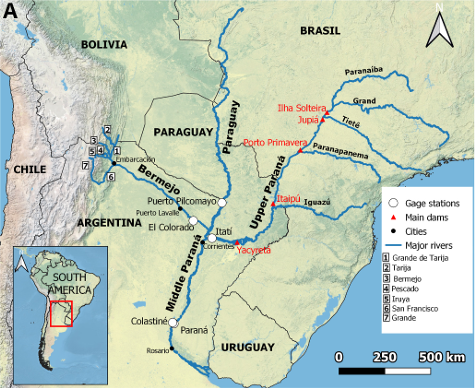
\includegraphics[width=0.65\linewidth]{figures/ch2/map rio parana.png}
    \caption{Rio Paraná  \textbf{(SOURCE?)}}
    \label{fig:rio parana map}
\end{figure}

%\begin{figure}[H]
 %   \centering
  %  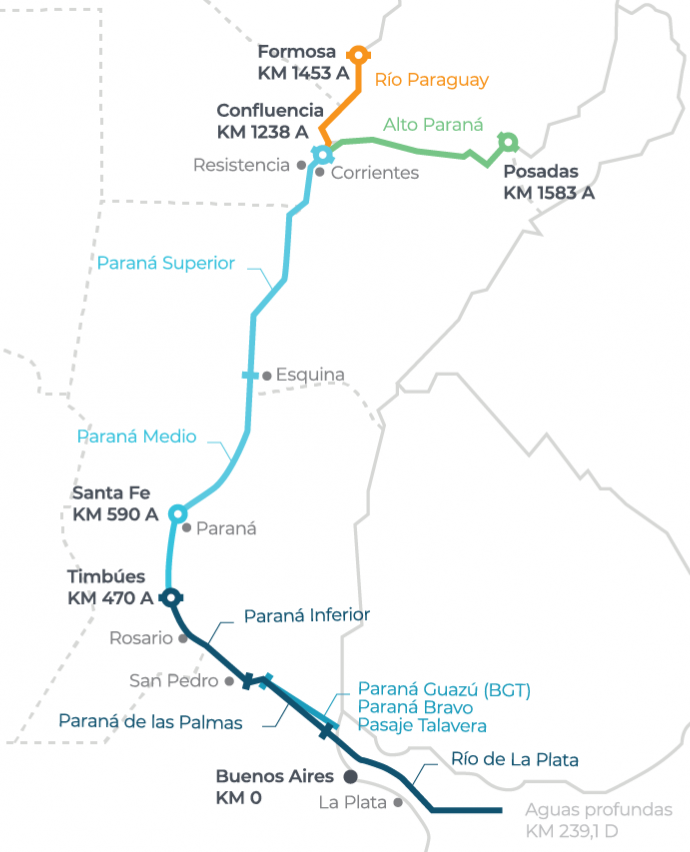
\includegraphics[width=0.5\linewidth]{figures/ch2/2025_mapa_vnt_extendida_tramos_profundidades_abril.png}
  %  \caption{The Vía Navegable Troncal (VNT) and the location of the Paraná and Paraná Guazú in it \autocite{agencianacionaldepuertosynavegacionNavegableTroncal2025}}
 %   \label{fig:VNT}
%\end{figure}

The Paraná river is formed by the junction of the rivers Grand and Paranaíba in south-central Brazil and flows for 4880 kilometers until it empties in the Río de la Plata near Buenos Aires, Argentina \autocite{orfeoHydraulicMorphologicalCharacteristics2002}. The river can be split up in three different sections: the upper, middle and lower Paraná. For these sections, the general characteristics related to discharge, channel size, and sediments are discussed.

The Upper Paraná River flows southwest, from the origin of the Paraná, until the confluence with the Paraguay river. Mean annual discharges at Porto São José, located near Porto Primavera at the confluence of the Paraná and Paranapanema in figure \ref{fig:rio parana map}, are between 6501 to 13,294 m³/s. The maximum flow velocity varies between 0.6–0.9 m/s in tributary channels and up to 1.4 m/s in the main channel during floods \autocite{stevauxUpperParanaRiver1994}. The Upper Paraná River exhibits a multi-channelled, braided pattern with numerous islands and sand bars, and its floodplain is strongly asymmetrical, being much wider on the right side (4.2–8.5 km) while the left margin erodes the Caiuá Formation \autocite{orfeoHydraulicMorphologicalCharacteristics2002}. During normal floods, water enters the floodplain through secondary and abandoned channels, producing slow and non-unidirectional flow, but extreme floods can cause crevasses and temporary channels. The channel is 1200–4500 m wide and 6–17 m deep with a slope of 0.096 m/km \autocite{stevauxUpperParanaRiver1994}. Finally, the suspended sediment concentration at Porto Rico, just South of Porto São José, equal 14.8×10\textsuperscript{6} tons/year and is mainly composed of quartz, mica, and kaolinite. The bed load at this location has a total discharge of 4.04×10\textsuperscript{6} tons/year and consists of quartz-rich (95\%) medium to fine sand \autocite{stevauxUpperParanaRiver1994}.

After the confluence with the Paraguay river, the Upper Paraná merges into the Middle Paraná River. This part of the river stretches until the start of the delta, just South of Rosario City. Near Corrientes City, South of the confluence, the mean annual discharge is 16,941 m\textsuperscript{3}/s, with summer floods (Feb–Mar) and spring low water levels, reaching maximum values above 50,000 m\textsuperscript{3}/s. The channel width ranges 1.9–4.7 km, with depths of 15–20 m and a slope of 0.085 m/km \autocite{orfeoHydraulicMorphologicalCharacteristics2002}. Below the Paraguay River confluence, suspended sediment concentrations are highly variable due to differences in discharge, confluence angle, and sediment characteristics between both rivers. The suspended solid concentration ranges from 18 to 554 mg/l, with the right margin showing much higher values (up to 1221 mg/l) than the left (maximum 88 mg/l)  \autocite{depetrisSuspendedLoadRio1968}. The suspended load is mainly silt (61–66\%) on the right margin and clay (79\%) on the left, with minor fine sand. The bed load is composed mostly of medium to fine quartz sand. The total sediment discharge is estimated at 158.4×10\textsuperscript{6} tons/year, with suspended load contributing 75\% of that \autocite{orfeoHydraulicMorphologicalCharacteristics2002}.

The final and smallest part of the Paraná is the Paraná delta, that ranges for around 320 kilometers, from Diamante, Entre Ríos, until the Río de la Plata near Buenos Aires. It is divided into three large regions: the Upper delta (from Diamante to Villa Constitución, Santa Fe province), the Middle delta (from Villa Constitución to Puerto Ibicuy, Entre Ríos province) and the Lower delta (from Puerto Ibicuy to the mouth of estuary called Río de la Plata). As mentioned in the introduction, this study focuses on the Lower delta specifically. Just upstream of the delta apex, near the city of Paraná, the mean annual discharge is 18,500 m\textsuperscript{3}/s with peak discharges up to 60,000 m\textsuperscript{3}/s \autocite{westerHydrodynamicModellingTidal2018}. Its width varies between 18 and 60 kilometres. The Paraná delta is characterized by many islands, which exist due to the large amounts of sediment that the Paraná delta carries: at its mouth it transports approximately a total of 160,000,000 tons of sediments per year. The particle load distribution is as follows: 25\% consists of clay, 60\% is silt and around 15\% can be characterized as sand \autocite{academialabParanaDelta}. This sediment is deposited in the joint Paraná and Uruguay estuary, the Río de la Plata.


\section{Origin of sediment content in Paraná Guazú}
\label{sec:origin sediment content}
In the previous section, the quantities and distributions of sediment transport were lined out. However, a key step in the construction of the sediment balance of the Rio Paraná Guazú, located in the Lower Paraná, is to identify the origin of its sediment. As shown in Figure \ref{fig:placeholder}, the Lower and Middle Paraná receive discharge from three main tributaries: the Bermejo, Paraguay, and Upper Paraná Rivers. The total average discharge in the Middle Paraná is 18,389 m\textsuperscript{3}/s, of which 78\% is supplied by the upper Paraná. \citeauthor{lopezweibelSourcesTemporalDynamics2022} report that the Bermejo contributes only 2\% of this discharge. Nevertheless, the Bermejo is the dominant source of sediment, due to intense erosion in the Andes Eastern Mountain Range within its basin. During the wet season (November to April), multiple tributaries in the basin contribute large sediment flows, accumulating to an annual suspended sediment load of $106 ~\times 10^6$ t per year at El Colorado gauge station. 

It is interesting to know that the contribution of sediment from the Bermejo to the Paraná is approximately 90\% today, but that this is in fact due to the installation of the Itaipu dam built in 1971, located in the south of Brazil just before the border with Argentina and Paraguay. This modification of the sediment voyage cuts a supply of about 50\% compared the initial amount of sediment, this 90\% used to be 56\% of the sediment income before the construction of the dam. This explains us that the human action already hindered the initial inflow of sediment a long time ago \autocite{hibaParanaRiverEcological2024}.

From all the sediment transported in the river only a fraction ends up at the end of the river, a section called 'the delta' \autocite{academialabParanaDelta}. A delta is a landscape formed at the mouth of a river where the water eventually runs into the ocean. At these locations, the water's velocity decreases, leading floating particles in the water to settle in the delta. These floating particles contain gravels, sands and clays which over time and distance are decreasing in particle size due to mutual erosion. This transport of sediment contributes to the sediment balance of the river. Besides that, deltas are also characterized by high vegetation growth. When this vegetation dies, the organic material will change into peat due to the governing pressures. So, in a delta one expects to find relatively soft soils (sands) and very soft soils (clay and peat). Dotted with islands, these wetlands are a source of ecosystem services such as flood and drought buffering, water purification, erosion control and coastal protection, climate regulation, as well as the provision of shelter, feeding and breeding sites for various wildlife species. For this reasons, rich biodiversity of the delta territory are characterised by the flora and fauna and the microorganisms living in the river. The sediment itself contains particles is used by the flora and fauna as nutrition and a filter system for the water quality. The microorganisms inside of the water also feed on it. 
Therefore, they can exist thanks to the transport of sediment, but are on the other hand also quite dependent on it\autocite{hibaParanaRiverEcological2024}.

In recent years, wetlands have become increasingly studied for their their key role against climate change. This is, for the number of reasons listed in the paragraph above, overall serving as natural barriers against floods and droughts, and also their function as carbon sinks. Despite the importance of the delta, the ecosystems remain under great threat from human action. It is estimated that globally, 85 percent of the wetlands that existed three centuries ago have been destroyed or drastically transformed \autocite{hibaParanaRiverEcological2024}.

In summary, while the Paraguay and Upper Paraná Rivers provide most of the fluvial discharge to the downstream delta, the Bermejo River delivers the majority of sediments \autocite{lopezweibelSourcesTemporalDynamics2022}. These sediments pass through the whole river channel, end up in the deltas while contributing to the biodiversity of the whole Parana region. Delta's are strategic ecological elements that need to be protected for the sake of the river's biodiversity and pollution indexes. For this reason, the stretch of river beginning in the Bermejo basin and continuing via the Paraguay and Middle Paraná to the Paraná Guazú is of particular importance in this study. 


\section{Types of sand mining}
In order to learn more about the effects that sand mining can cause, the general procedure of mining sand should be explained. Due to the significant demand of sand in human society, various techniques have been established to extract. This can be done through so-called dry sand mining, where sand is won from the land, or through river sand mining. For the river extraction, the focus lies on in-stream mining. Both processes are relevant for the study and therefore explained in the following paragraph.

In-stream mining is the extraction of sand and gravel from the active channel of a river \autocite{sand-mining-boek}. A number of types of in-stream dredging exist. Bar scalping or skimming is the most common extraction practice, consisting of removing the lower two thirds of a bar while leaving the top third to minimize alteration of the riverbed’s initial conditions. Dry pit channel mining involves creating a dry pit using mechanical or manual tools to extract sand or gravel; the remaining pits act as head cuts that modify upstream flow during high-water seasons. Wet pit channel mining, typically carried out in perennial rivers, produces similar effects and damages as the dry pit method. Bar excavation takes place downstream of a bar to capture sand and gravel being transported by the current. Finally, in-stream traps involve digging a hole to collect sediment during high flow periods, which can later be retrieved once water levels drop \autocite{sand-mining-boek}.

\section{Purposes of the extracted sand}
Creating a clear understanding of the sand extraction processes is key for the study. This highly contributes understanding the bigger picture of potential problems and stakeholder relations. For this reason, one shall also reflect on the purpose of the sand extraction, which will be done in the following text. 

The extracted sand can be used for different reasons. Historically, silica sand was used as a raw material for the glass industry, as well as the construction industry for the cement creation but since the introduction of fracking, sand miners have found a new attractive market for their product. The exact volumes of sand used for fracking versus the volumes used for other purposes are unknown. However, as seen in Figure \ref{fig:sanddiagram}, the rising trend in sand production can be observed only for the past years, after the discovery of Vaca Muerta.

In the 1970's, geologists became increasingly aware that large volumes of gas existed in low-permeability sandstones. However, conventional methods did not allow for economic extraction of gas from these `tight reservoirs' \autocite{lawGasTightReservoirs1992}. Hydraulic fracturing, also called 'fracking', is a method that was first tested in 1947 and then applied on large scale in the 1970's. It is used to extract oil and natural gas from these low-permeability rock formations, shale formations being the primary example \autocite{denchakFracking1012019}. The technique starts by drilling a long vertical well. As soon as the desired rock formation is reached, drilling gradually turns horizontal and steel pipes called `casings' are inserted into the well. Small holes are perforated in the casing and then fracking fluid is pumped in at a pressure high enough to create new fractures or open existing ones in the surrounding rock. This allows previously unavailable oil or gas to flow to the surface \autocite{denchakFracking1012019}.

The fracking fluid contains as much as 97\% of water, and the leftover 3\% are called 'proppants'. These proppants are small, solid particles that keep the fractures in the rock formation open after the pressure from injection is removed. Sand, or more specifically silica sand, is the most widely-used proppant in the fracking industry \autocite{denchakFracking1012019}. Sand is thus an essential substance to keep the drilled pores open and to allow for the fossil fuels to flow out.


\section{The effects of sand mining}
Existing literature provides a framework for possible effects that arise due to river sand mining. This framework helps to determine the exact effects of dredging in the Paraná delta.

As mentioned previously, rivers maintain an equilibrium between erosion, transport, and deposition of sediments. However, instream sand mining can disrupt this balance. This happens through direct disruption of the channel geometry or through so-called incision and related undercutting of banks \autocite{sand-mining-boek}. The direct disruption of the river bed depends on the type of sand mining technique employed. In the case of pit excavation, the river bed is locally lowered and a so-called 'nick point' is created. With bar skimming the river bed is widened \autocite{sand-mining-boek}. For the remainder of this section, the consequent effects of the local river bed lowering (the nick point) are discussed.

Channel incision causes the nick point to migrate both upstream and downstream. In the case of high flows, due to its shape, the nick point is the point where most erosion occurs. Water plunges over the step and erodes the bed at the base. As flows continue, the drop migrates upstream, a process which is often called head-cutting in literature. On the other hand, a process called 'hungry water' causes downstream migration of the pit \autocite{sand-mining-boek}. At the mining pit the water level is deeper, which causes the flow velocity to reduce locally. This leads to a decrease in flow energy and thus to more deposited sediment. When the flow leaves the mining area, water levels are shallower again meaning that flow velocity and energy significantly increase. A lot of sediment has been deposited in the nick point, meaning that the water is not using its full sediment carrying capacity anymore. In other words, the water is 'hungry' for sediment and erosion downstream increases \autocite{sand-mining-boek}. 

Through the combined effects of head-cutting and hungry water, the mining pit can extend beyond the initial dimensions caused by direct disruption. This happens in both downstream and upstream directions, as summarized in figure \ref{fig:channelbedeffects}. \textcite{hackneyRiverBankInstability2020} have demonstrated that sand mining has the potential to lower bed levels sufficiently to
cause river bank instability.

\begin{figure}[H]
    \centering
    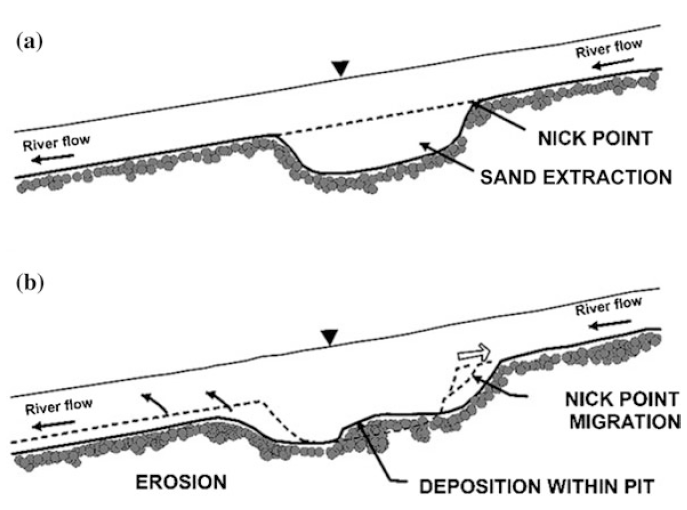
\includegraphics[width=0.75\linewidth]{figures/channelbedeffects.png}
    \caption{(a) direct disruption leads to a locally lowered water bed. (b) channel incision makes the pit migrate upstream through head cutting and downstream through 'hungry' water \autocite{sand-mining-boek}}
    \label{fig:channelbedeffects}
\end{figure}

Previous studies have shown that bed coarsening can also occur as a result of sand-mining. Fine particles are removed, leading to a greater concentration of coarse, close to gravel, particles. This effect can also be seen upstream \autocite{sand-mining-boek}. Further, sand mining can lead to changes in both water quality and quantity. The process of dredging the fine sand stirs fine organic and inorganic particles, thereby increasing the turbidity of the water. This reduces light penetration, which means less photosynthesis and ultimately less organic growth in the water \autocite{sharipEffectsSeasonSand2014}.

As mentioned before, mining pits are often places with significant deposition of particles. Fine, nutrient-rich particles can settle and get trapped in the pits. This then reduces the transport of nutrients from the river to the coastal waters \autocite{sand-mining-boek}. Concerning the water quantity, the most relevant effects are related to the groundwater: the lowering of the river bed through direct disruption or channel incision can lead to a lower groundwater table. This can lead to settlements or have negative effects on flora and fauna surrounding the river \autocite{rentierEnvironmentalImpactsRiver2022}.

\section{River bank stability}
Following the study on the effects of sand mining on the river bed, it is relevant to look at the effects on the river banks. Dry sand extraction does not influence the bank stability unless the location of extraction is the river bank itself. Therefore, this section only concerns the topic of river sand extraction.
River sand mining can create instabilities in the river bed as shown in the previous section. This can potentially act on the river banks because of the fact that the river channel goes deeper, influencing the discharge and increasing its water influence on the banks \autocite{hackneyRiverBankInstability2020}. In general, there are several ways that the water has potential negative impacts on the river bank. Bank failure can be caused by house placement, soil saturation, weight on the river bank, vegetation and tectonic events; but most of them are due to the variation of the water level and waves. The reason behind this is that the river bank is naturally eroded when the water exerts a force on it \autocite{governmentofsouthaustraliaRiverbankCollapse2024}.
The river bank is divided in three parts: the toe, the bank and the overbank zone. The toe of the bank is the most susceptible to erosion when in contact with high water levels, which can be seen in the Figure \ref{fig:Effect of Water on Bank after One Year}.

\begin{figure}[H]
    \centering
    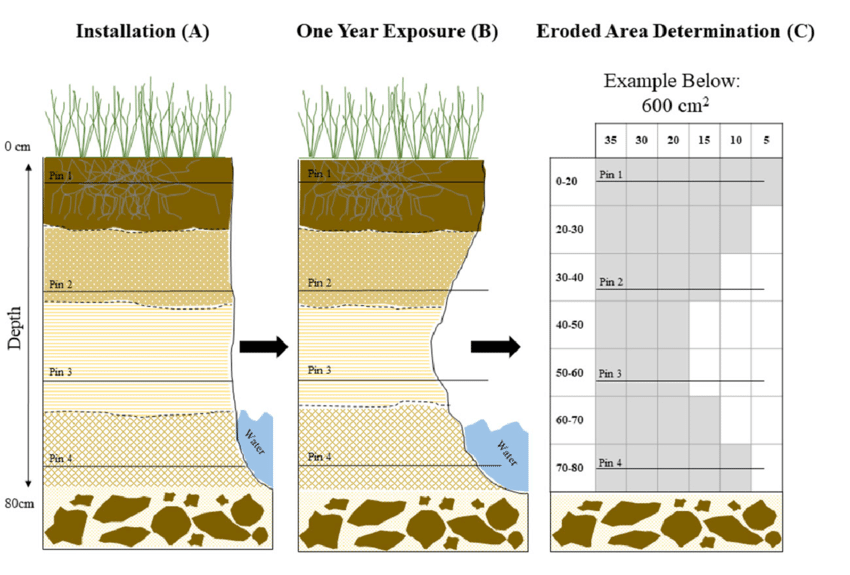
\includegraphics[width=0.5\linewidth]{figures/ch2/Erosion.png}
    \caption{Effect of water on bank after one year \textbf{(SOURCE?)}}
    \label{fig:Effect of Water on Bank after One Year}
\end{figure}

When the combination of high water level with a strong current is highest, the bank zone is affected by the tidal currents or waves. This is because, as seen in Figure \ref{fig:Effect of Water on Bank after One Year}, water erodes the layer of the bank where the extra water level pushes, creating a dent inside the soil layer.
Consequently, after some time the upper overbank area has less and less support underneath, thus becoming unstable and collapsing. 
Repeating this process takes the river bank further inside the land, increasing the channel width and absorbing the land near the river bank. 

Finally, it must be noted that the effects of sand mining can be diverse: previous studies have shown negative impacts on biodiversity, including reduced benthic fauna, disrupted fish spawning habitats, and depletion of natural mosquito predators such as dragonflies \autocite{sand-mining-boek}. The socioeconomic effects of mining can vary, in the short-term it often provides employment, income, and government revenue through royalties and taxation. However, in the long-term the operation can cause a reduction in access to clean water and can cause water scarcity, especially in dry periods. Additionally, loss of land and access to land together with loss of trees and vegetation can jeopardize the local food security. Finally, infrastructure can be damaged by the lowering of the river bed and/or the groundwater table \autocite{sand-mining-boek}.

\section{Nature-based solutions}
 NbS align with the broader goals of climate resilience and sustainable development. The exploration of nature-based solutions (NbS) is not only timely but essential for the Paraná Guazú and its surrounding ecosystems. As highlighted in the preceding sections, the Paraná Guazú located within the Lower Paraná delta could face significant environmental pressures due to sand mining. The ecological and socioeconomic consequences of these disruptions underscore the need for sustainable mitigation strategies that go beyond traditional engineering approaches. As a start, one may read the general definition of Nature-based solutions:

\textit{“A set of actions to protect, conserve, restore, sustainably
use and manage natural or modified terrestrial, freshwater, coastal and marine
ecosystems, which address social, economic and environmental challenges
effectively and adaptively, while simultaneously providing human well-being,
ecosystem services, resilience and biodiversity benefits” \autocite{eiselinVerenigdeNatiesStemmen2022}}

Nature-based solutions is an initiative launched by International Union for Nature Conservancy (IUCN) at the start of the 21st century \autocite{cassinChapter2History2021}. Its aim is to fulfil the 7 Goals set by the IUCN found in the Figure \ref{fig:7g} \autocite{dunlopEvolutionFutureResearch2024}.

Implementations of NbS often face resistance from stakeholders, particularly when these solutions are compared to traditional engineered approaches. This resistance stems from several key factors:
\begin{itemize}
    \item Lack of knowledge: local communities and stakeholders may be sceptical of NbS due to their less straightforward approach compared to conventional infrastructure such as concrete walls or revetments. The abstract or long-term benefits of NbS such as ecosystem restoration, flood regulation, or biodiversity enhancement can be harder to accept as a plan.
    \item Natural uncertainties: NbS often rely on natural processes, which can introduce risks in terms of feasibility and maintenance. Stakeholders may question whether these solutions can deliver the same level of protection or economic return as traditional non sustainable engineering solutions.
    \item Economical rentability: a decent return of investment is essential for securing funding and support from investors. Without clear evidence of effectiveness and other financial benefits, stakeholders such as investors, mayors, and community leaders may hesitate to choose this path.
\end{itemize}

If solutions are presented, they must be clear, easy to implement and without a lot of financial constraints. Otherwise, without funding of the project there is no execution.

\begin{figure}[H]
    \centering
    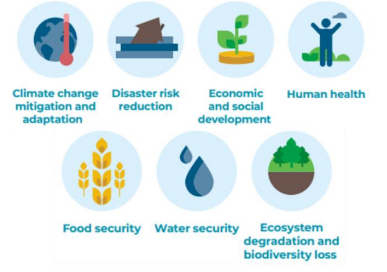
\includegraphics[width=0.50\linewidth]{figures/ThesevenNBSgoals.png}
    \caption{Seven goals for achieving a good NbS \autocite{dunlopEvolutionFutureResearch2024}}
    \label{fig:7g}
\end{figure}